\documentclass[runningheads]{../llncs}

\usepackage{subcaption}
\usepackage{tabularx}
\usepackage{multirow}
\usepackage{booktabs}
\usepackage[export]{adjustbox}
\usepackage{array}
\newcolumntype{L}[1]{>{\raggedright\let\newline\\\arraybackslash\hspace{0pt}}p{#1}}
\newcolumntype{C}[1]{>{\centering\let\newline\\\arraybackslash\hspace{0pt}}p{#1}}
\newcolumntype{R}[1]{>{\raggedleft\let\newline\\\arraybackslash\hspace{0pt}}p{#1}}

% Used for displaying a sample figure. If possible, figure files should
% be included in EPS format.
\usepackage{graphicx}
\graphicspath{{../images/}}

% If you use the hyperref package, please uncomment the following line
% to display URLs in blue roman font according to Springer's eBook style:
\usepackage[colorlinks=true, linkcolor=blue, urlcolor=blue, citecolor=blue, anchorcolor=blue]{hyperref}
\renewcommand\UrlFont{\rmfamily}

\begin{document}

\title{Learning Grasp Evaluation Models Using Synthetic 3D Object-Grasp Representations}

\titlerunning{Learning Grasp Evaluation Models}
% If the paper title is too long for the running head, you can set
% an abbreviated paper title here
%
\author{
    Minh Nguyen \inst{1} \and
    Paul G. Pl\"{o}ger \and
    Alex Mitrevski\inst{1} \and
    Maximilian Sch\"{o}bel\inst{1}}
%
\authorrunning{M. Nguyen et al.}
% First names are abbreviated in the running head.
% If there are more than two authors, 'et al.' is used.
%
\institute{Hochschule Bonn-Rhein-Sieg, Grantham-Allee 20, 53757 Sank Augustin, Germany \\
\email{minh.nguyen@smail.h-brs.de}, \email{\{paul.ploeger,aleksandar.mitrevski,maximilian.schoebel\}@h-brs.de}}
%
\maketitle              % typeset the header of the contribution

\begin{abstract}
This project considers the problem of generating data for training grasp evaluation models. Recent advances are reviewed
for four main aspects most relevant to labeled grasp data synthesis, namely feature extraction from perceptual data,
object-grasp representation, grasp evaluation techniques, and data generation techniques. From this review, one may
conclude that while data synthesis for learning a grasp evaluation model is promising, recent approaches are either
limited by difficulties in collecting large-scale human grasp experience, or by the shortcomings of using analytical
metrics to label generated data. Additionally, a completed object grasping pipeline is integrated, from object
detection to grasp pose detection and grasp execution. Two set of experiments are performed on the Toyota Human Support
Robot for two pose estimation methods using this grasping pipeline. The pipeline proves reliable and fast enough for
performing the experiments, being able to execute 20 grasps per object without interruption. While further extension and
optimization are needed, the pipeline enables directly examining and comparing more advanced grasp planning methods in
the future.

\keywords{Grasp learning \and Data synthesis.}
\end{abstract}

%%%%%%%%%%%%%%%%%%%%%%%%%%%%%%%%%%%%%%%%%%%%%%%%%%
\section{Introduction}

%%%%%%%%%%%%%%%%%%%%%%%%%%%%%%
\subsection*{Motivation}

\begin{figure}[h!]
    \centering
    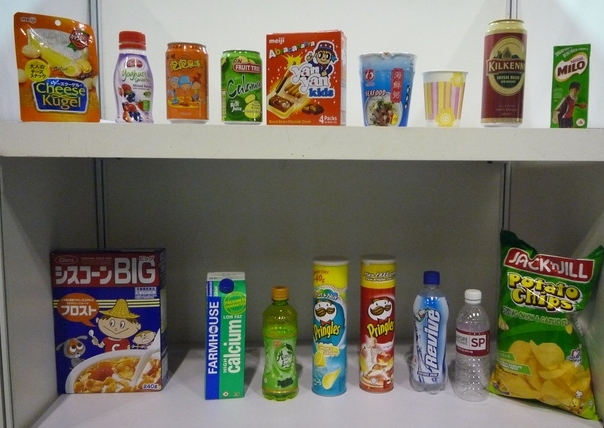
\includegraphics[width=0.5\textwidth]{robocup_typical_objects}
    \caption{Typical objects in the Robocup@Home competition \cite{robocupRulebook2018}.}
    \label{fig:robocup_objects}
\end{figure}

Robot grasping with multi-fingered robotic hands is a challenging problem, and finding a grasp planning solution which
resembles humans' grasps in dexterity and robustness is still an area of active research. This project focuses on
grasping tasks relevant to the Robocup@Home competition \footnote{\url{http://www.robocupathome.org}}. These tasks
involve typical objects in a domestic environment, some of which can be seen in figure \ref{fig:robocup_objects}. The
grasp experiments described in section \ref{section:experiments} will be conducted on the Human Support Robot (HSR)
from Toyota \footnote{\url{https://www.toyota-global.com/innovation/partner_robot/robot/}}.

%%%%%%%%%%%%%%%%%%%%%%%%%%%%%%
\subsection*{Overview of robotic grasping}

Figure \ref{fig:grasp_synthesis_mind_map} outlines the aspects relevant to generating a grasp strategy for an arbitrary
object. Grasp synthesis approaches are generally classified as either analytical or empirical \cite{Sahbani2012}.
Analytical methods typically consider the following mechanical properties of the contact points between the gripper's
fingers and an object \cite{Roa2015,Sahbani2012,Shimoga1996}: disturbance resistance, dexterity, equilibrium and
stability. Empirical approaches, on another hand, typically rely on some form of grasp experience for learning to
evaluate grasp candidates. Bohg et al. \cite{Bohg2014} further categorize these methods based on how much information
is assumed about the object: whether they are known, familiar or completely unknown to the robot.

\begin{figure}[h!]
    \centering
    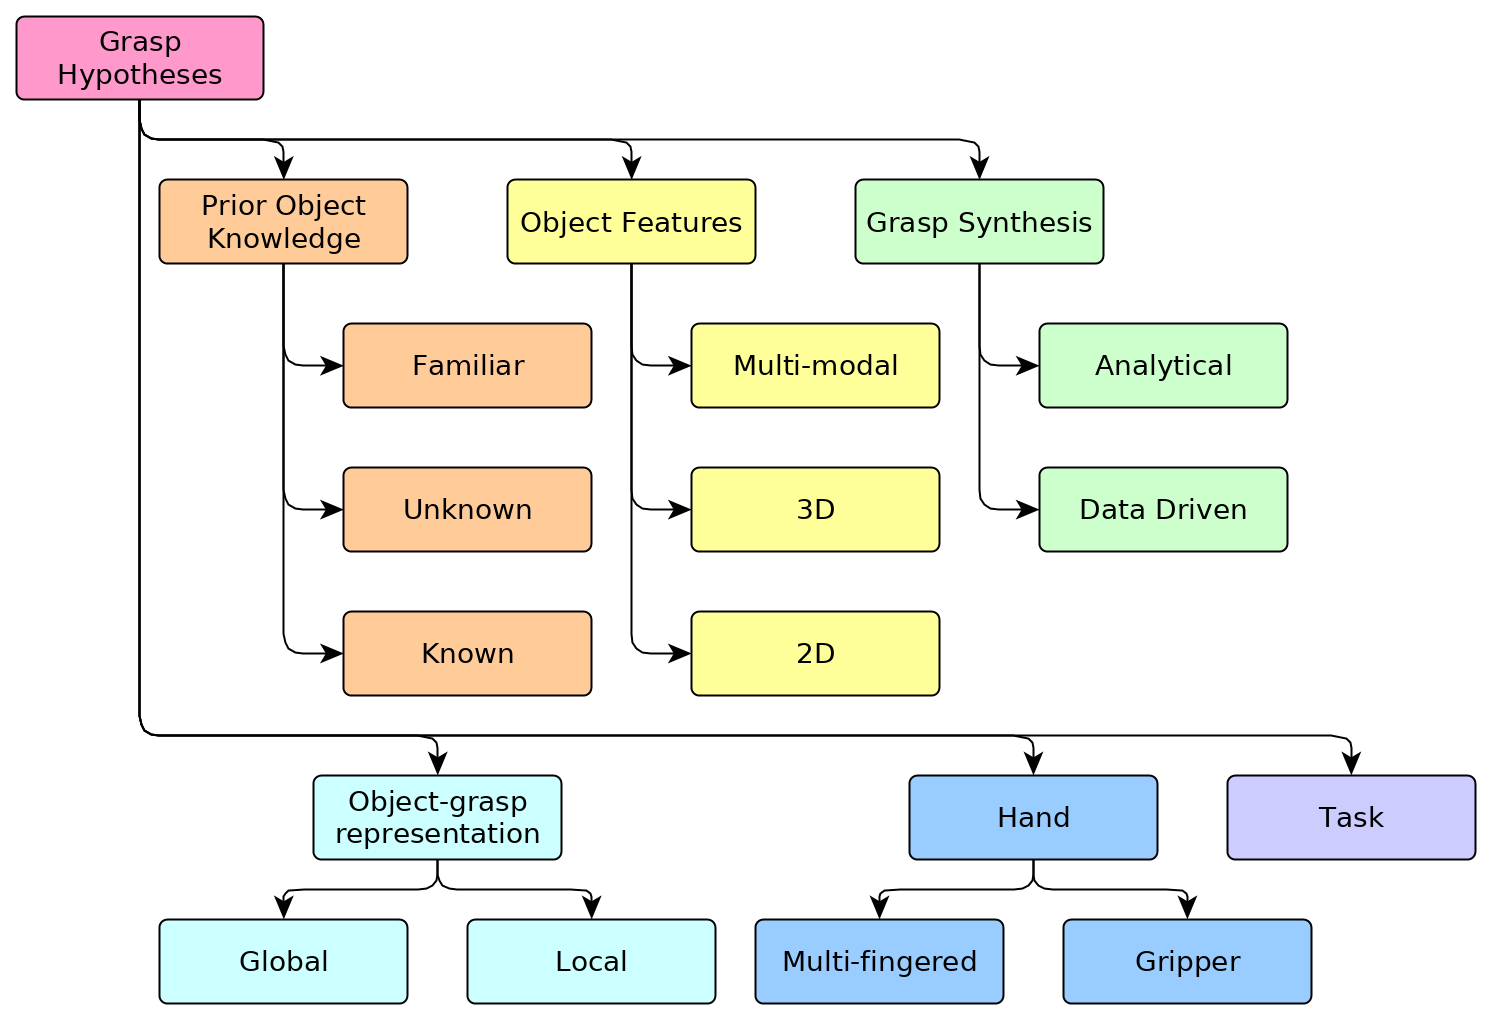
\includegraphics[width=0.9\textwidth]{bohg14-grasp_synthesis_mind_map}
    \caption{Aspects which may influence generation of grasp hypotheses \cite{Bohg2014}.}
    \label{fig:grasp_synthesis_mind_map}
\end{figure}

Because of their dependence on knowledge about the object, the end-effector and the environment, which maybe missing
or incomplete in real world applications, analytical methods have been shown to be unreliable in synthesizing stable
grasps when applied on real robots \cite{Kappler2015,Rubert2017,WeiszAllen2012}. Grasping data, however, are
time-consuming and costly to collect. In this context, the next section will discuss recent advances in fields relevant
to synthesizing data for training grasp evaluation models, specifically: how to extract features from perceptual data,
how to represent object-grasp relations from these features, how to evaluate these representations, and how to
synthesize and augment grasp datasets.

%%%%%%%%%%%%%%%%%%%%%%%%%%%%%%%%%%%%%%%%%%%%%%%%%%
\section{Advances in aspects relevant to empirical grasp synthesis}

%%%%%%%%%%%%%%%%%%%%%%%%%%%%%%
\subsection{Feature extraction from perceptual data for grasping}

RGB-D cameras are becoming the perceptual sensor of choice for robotic systems because of their richer features
compared to pure RGB images \cite{lenz2015,Eitel2015,Gupta2014RGBDFeatures,jiang2011}, especially in the context of
grasping where 3D information of an object's surface heavily influences how it can be grasped. Extracting features from
RGB-D data often requires consideration of their inherent multi-modality. Bo et al. \cite{Bo2013} build sparse coding
dictionaries for RGB-D data using the K-SVD algorithm and propose to use a hierarchical matching pursuit (HMP)
algorithm to compute a feature hierarchy for new RGB-D images. Lenz et al. \cite{lenz2015} use deep auto-encoders to
build a representation for each feature channel, then introduce ``structured regularization'' to combine the depth and
color representations.

More recent approaches leverage the success of Convolutional Neural Networks (CNN) in image processing for extracting
features from RGB-D data. Gupta et al. \cite{Gupta2014RGBDFeatures} propose the HHA representation, which encodes the
depth each pixel of the depth image with horizontal disparity, height above ground, and the angle between the local
surface normal and direction of gravity. Eitel et al. \cite{Eitel2015} propose to use convert the depth value directly
into RGB values using a jet color mapping. Porzi et al. \cite{Porzi2017} introduce a convolutional block called
\emph{DaConv} to learn scale awareness using depth information.

Instead of projecting RGB-D data onto different feature channels, several methods are developed to deal with 3D
information directly, via training either a volumetric CNN architecture or multiple CNN models from different
perspectives on data generated from object meshes in simulation. Notably, Qi et al. \cite{Qi2016} develop two novel
volumetric CNN architectures and extend the multi-view CNN technique proposed by Su et al. \cite{Su2015} for object
classification.

Techniques are also developed to deal with occluded regions in point clouds. Bohg et al. \cite{Bohg2011MindTheGap}
search for a symmetric plane perpendicular to the workspace surface (i.e. table) and mirror the incomplete point cloud
across this plane to fill in the missing information. Varley et al. \cite{Varley2017} train a CNN to predict whether
the obscured cells in an occupancy grid are occupied.

%%%%%%%%%%%%%%%%%%%%%%%%%%%%%%
\subsection{Object-grasp representation}
Bohg et al. categorizes object-grasp representations into ones using local (i.e. curvature, contact area with the hand)
or global features (center of mass, bounding box).

\subsubsection*{Techniques based on global features.}

Ciocarlie and Allen \cite{Ciocarlie2009} introduce Eigengrasps and defined them as principal components of the dataset
of human hand configurations. The Eigengrasp planner is proposed where a quality metric are optimized for the Eigengrasp
representations of grasp candidates. The planner is also used by Goldfeder and Allen \cite{Goldfeder2011} to synthesize
a grasp dataset for object models. Mahler et al. \cite{mahler2017} represent grasps in 2D images by aligning the image
center to the gripper central point and the image's middle row to the grasp axis. The grasp is assumed to have an
approach vector perpendicular to the table and hence can be characterized by the gripper center and the angle of the
gripper axis with respect to the table.

\subsubsection*{Techniques based on local features.}

Several methods represent grasp candidates for bipedal gripper as rectangles positioned in RGB and/or depth images at
contact point with the object \cite{jiang2011,Detry2012,lenz2015}. Features extracted from the RGB-D image regions
within these rectangles are then used to train a model (e.g. Multilayer Perceptron (MLP) \cite{lenz2015} or CNN
\cite{jiang2011}) to evaluate the respective grasp candidates.

Kappler et al. \cite{Kappler2015} extract local shape representations (or templates) as projection of the objects'
point clouds onto grids with a predefined resolution. These grids are aligned with the plane tangent to the object
surface at the intersection point between the grasp approach vector and the object.

Gualtieri et al \cite{Gualtieri2016} propose to represent a grasp candidate by the cuboid swept out by a two-fingered
gripper as it closes on the object, where the occluded points are sampled. The regions are voxelized into $60 \times 60
\times 60$ grids and projected onto three orthogonal planes to create 15 channels before being used as input for a CNN
grasp evaluation model.

%%%%%%%%%%%%%%%%%%%%%%%%%%%%%%
\subsection{Grasp evaluation}

\subsubsection*{Analytical grasp metrics.}

Roa and Su{\'a}rez \cite{Roa2015} group analytical grasp quality measures into approaches focusing on contact point
position, hand configuration, and ones which combine both metric types. Contact point grasp quality measures focus on
the object's properties, friction constraints, and form/force closure conditions, most often via analyzing properties
of the grasp matrix $ G $ or the grasp wrench space (GWS) $ \mathcal{P} $. Methods focusing on hand configuration often
extends metrics calculated from $ G $ to the hand-object Jacobian $ H $. Analytical metrics can be extended to consider
task affordance via limiting the analysis to only movements relevant to performing a specific task.

Most popular among analytical metrics is the $ \epsilon $-metric (also known as the ball metric). The metric can be
geometrically characterized by the radius of the largest sphere that can be contained in $ \mathcal{P} $ and centered
at its origin \cite{Roa2015}. Weisz and Allen \cite{WeiszAllen2012} extend the $\epsilon$-metric by introducing noise
to object pose in simulations and rating grasp candidates by the probability that they obtain a certain
$ \epsilon $-metric score for all pose perturbations. Evaluation using this extension shows that grasps with the best
$ \epsilon $ score is much more likely to have low $ \epsilon $ score when pose variations are introduced. While the
proposed approach is more robust to pose uncertainty, calculation of the metric is intractable in real time.

\subsubsection*{Learning to predict grasp quality.}

Table \ref{table:grasp_approaches} summarize the most recent and prominent approaches to training a grasp evaluation
model. Jiang et al.'s \cite{jiang2011} trains an SVM model to learn the weight matrices which linearly combine
pixel-wise values of numerous filters of the original RGB-D data to produce a final grasp quality score. Lenz et al
\cite{lenz2015} use auto-encoders as feature extractors from RGB-D point clouds and use the encoder weights to
initialize the MLP model before training it to predict the probability of success for grasp candidates. More recent
approaches \cite{Kappler2015,Gualtieri2016,mahler2017} train CNN models directly on 2D projections or filters of their
object-grasp representations to produce a grasp quality value.

\begin{table}[h!]
    \scriptsize
    \def\arraystretch{1.2}
    \begin{tabularx}{\linewidth}{L{0.05\linewidth}C{0.39\linewidth}L{0.28\linewidth}L{0.28\linewidth}}
        Method & Object-grasp\linebreak representation & Feature extraction \& learning model & Data generation \\
        \toprule

        \cite{jiang2011}    & 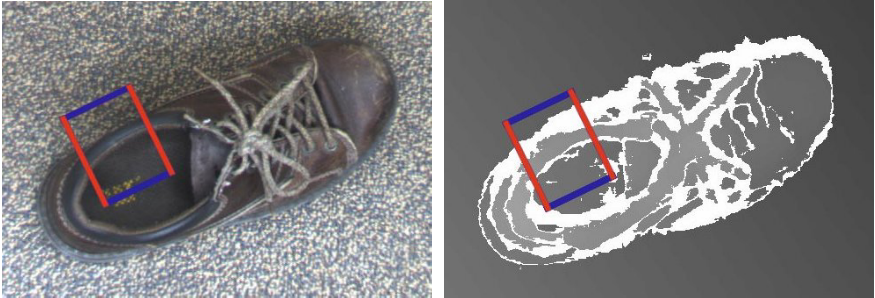
\includegraphics[scale=0.09,valign=t]{jiang_et_al-2011-grasp_representation}
            & Histogram of hand-crafted filters; \linebreak Model: SVM.
            & Rectangles manually \linebreak annotated. \\

        \cite{lenz2015}     & 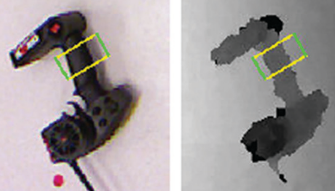
\includegraphics[scale=0.16,valign=t]{lenz_et_al-2015-grasp_representation}
            & Auto-encoders to initialize weights, structured regularization to combine depth and RGB data;
            \linebreak Model: MLP. & Extension of the \linebreak dataset from \cite{jiang2011} \linebreak (above). \\

        \cite{Kappler2015}  & 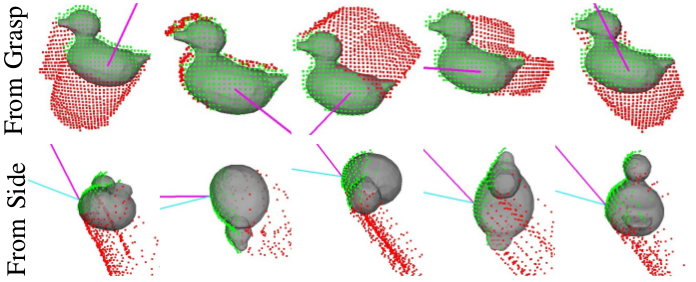
\includegraphics[scale=0.16,valign=t]{kappler_et_al-2015-fig8-local_shape_diff_viewpoints}
            & RGB rendering of ``template grids''; \linebreak Model: LeNet CNN
            & Quality of grasps are \linebreak calculated in simulation \linebreak for object meshes,
            \linebreak verified via crow-sourcing. \\

        \cite{Gualtieri2016}& 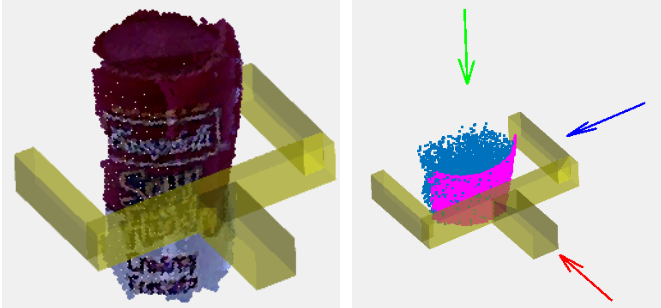
\includegraphics[scale=0.1,valign=t]{Gualtieri_et_al-2016-grasp_representation}
            & Filters of cuboid regions projected onto 3 orthogonal planes, creating 15 channels;
            \linebreak Model: LeNet CNN.
            & Quality of grasps are \linebreak calculated for object \linebreak meshes using force-closure \\

        \cite{mahler2017}   & 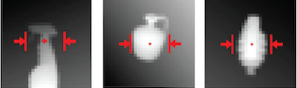
\includegraphics[scale=0.22,valign=t]{mahler_et_al-2017-grasp_representation}
            & Depth images cropped and aligned to gripper; \linebreak Model: CNN combined with single-layer NN.
            & Quality of grasps are \linebreak calculated for object \linebreak meshes using a variant of
            $ \epsilon $-metric from \cite{WeiszAllen2012} \\
        \bottomrule
    \end{tabularx}
    \caption{\small Five recent empirical approaches to grasp quality prediction}
    \label{table:grasp_approaches}
\end{table}

%%%%%%%%%%%%%%%%%%%%%%%%%%%%%%
\subsection{Generating data for grasp success prediction}
\begin{itemize}
    \item Data synthesis for robot grasping
    \item Data augmentation
\end{itemize}

%%%%%%%%%%%%%%%%%%%%%%%%%%%%%%%%%%%%%%%%%%%%%%%%%%
\section{Methodology}

%%%%%%%%%%%%%%%%%%%%%%%%%%%%%%
\subsection{Object detection}

\begin{figure}[h!]
    \centering
    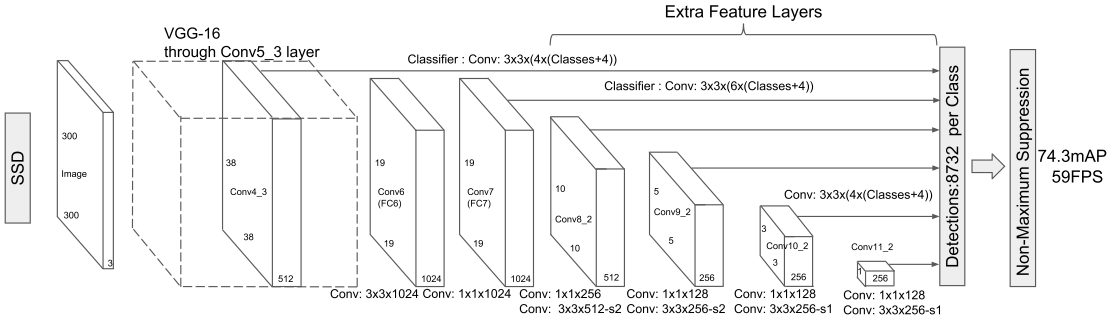
\includegraphics[width=\textwidth]{liu_et_al-2016-ssd_arch}
    \caption{SSD architecture \cite{Liu2016SSD}.}
    \label{fig:ssd_arch}
\end{figure}

Integrate Single-Shot Multibox Detector (SSD) for object detection (figure \ref{fig:ssd_arch})

%%%%%%%%%%%%%%%%%%%%%%%%%%%%%%
\subsection{Pose estimation and grasping}
\subsubsection*{Baseline method}
\begin{figure}[h!]
    \centering
    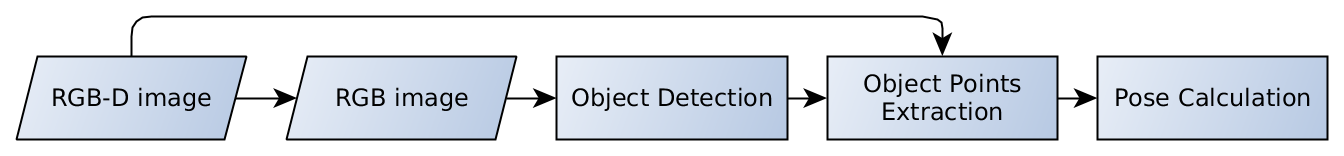
\includegraphics[width=\textwidth]{grasp_plan_pose_estimation}
    \caption{Flowchart of the baseline method for grasp experiments.}
    \label{fig:grasp_plan_baseline}
\end{figure}

\begin{itemize}
    \item assume the grasp approach to be along the $ x $-axis of the robot
    \item extract object points using image detection result
    \item estimate object positions in the \texttt{base\_link} coordinate frame
    \item estimated $ y $- and $ z $-coordinates are mean of the object points
    \item estimated $ x $-coordinate is either the minimum or mean of the object points
\end{itemize}

\subsubsection*{Grasp Quality CNN (GQCNN)}
\begin{figure}[h!]
    \centering
    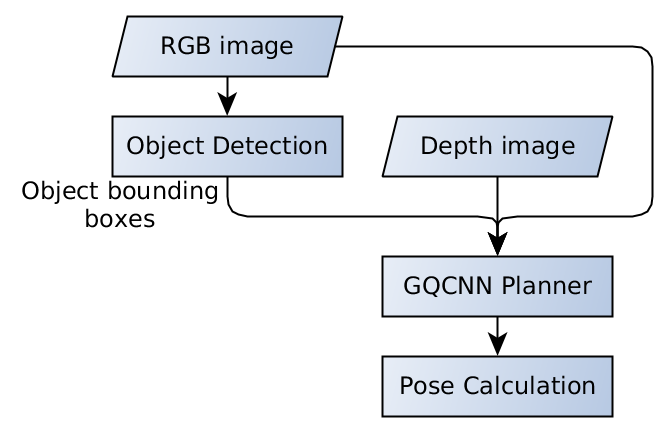
\includegraphics[width=0.5\textwidth]{grasp_plan_gqcnn}
    \caption{Flowchart of the integrated GQCNN grasp planner \cite{mahler2017}.}
    \label{fig:grasp_plan_gqcnn}
\end{figure}

\begin{itemize}
    \item GQCNN model \cite{mahler2017} is trained on Dex-Net 2.0 dataset to predict grasp robustness,
    \item In the original setup, the grasp is assumed to be from above and perpendicular with the table,
    \item Grasp approach vector is assumed to align with camera axis,
    \item Not reliable enough for performing grasp experiments.
\end{itemize}

\begin{figure}[h!]
    \centering
    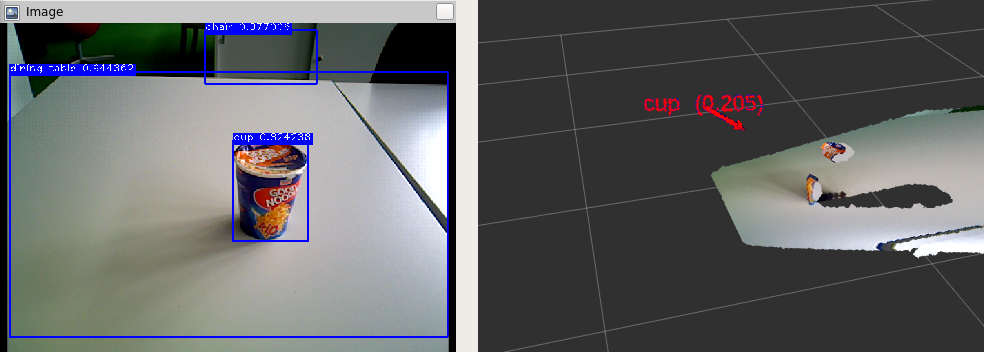
\includegraphics[width=0.9\textwidth]{grasp_gqcnn_result}
    \caption{A successful GQCNN grasp plan. Arrow and number on the right indicate grasp pose and quality returned from
             the GQCNN planner.}
    \label{fig:gqcnn_result}
\end{figure}

%%%%%%%%%%%%%%%%%%%%%%%%%%%%%%%%%%%%%%%%%%%%%%%%%%
\section{Experiments} \label{section:experiments}

%%%%%%%%%%%%%%%%%%%%%%%%%%%%%%
\subsection{Experimental Setup}

\begin{itemize}
    \item Two sets of experiments are performed for the variances of the baseline method described in slide
    \item Before each grasp, the robot is moved to a marked position facing the dining table.
    \item Objects further than 90cm in $ x $-axis and lower than 75cm in $ z $-axis are ignored.
    \item We use the SSD model pre-trained on the COCO dataset.
    \item Arm collisions and object slips are counted as failures.
    \item Only one of the objects in figure \ref{fig:objects} is grasped at a time.
\end{itemize}

\begin{figure}[h!]
    \centering
    \begin{subfigure}[t]{0.23\textwidth}
        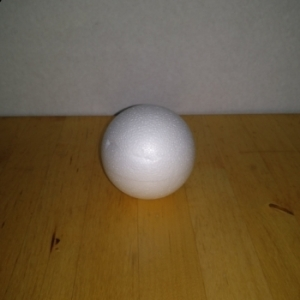
\includegraphics[width=\textwidth]{object_ball}
        \caption{\scriptsize Styrofoam ball}
        \label{fig:object_ball}
    \end{subfigure}
    ~
    \begin{subfigure}[t]{0.23\textwidth}
        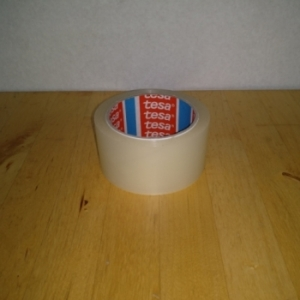
\includegraphics[width=\textwidth]{object_duct_tape}
        \caption{\scriptsize Duct tape}
        \label{fig:object_duct_tape}
    \end{subfigure}
    ~
    \begin{subfigure}[t]{0.23\textwidth}
        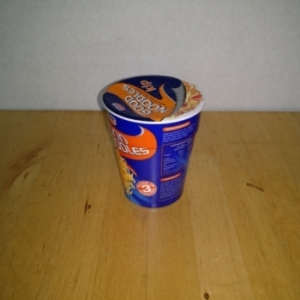
\includegraphics[width=\textwidth]{object_noodle_box}
        \caption{\scriptsize Noodles box}
        \label{fig:object_noodle_box}
    \end{subfigure}
    ~
    \begin{subfigure}[t]{0.23\textwidth}
        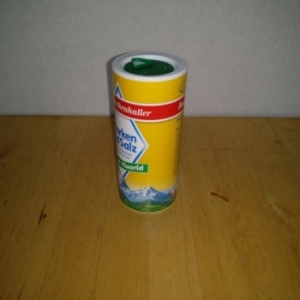
\includegraphics[width=\textwidth]{object_salt}
        \caption{\scriptsize Salt container}
        \label{fig:object_salt}
    \end{subfigure}
    \caption{Objects selected for the experiments.}\label{fig:objects}
\end{figure}

%%%%%%%%%%%%%%%%%%%%%%%%%%%%%%
\subsection{Results}

\begin{table}[h!]
    \centering
    \begin{tabularx}{\textwidth}{L{0.3\textwidth}C{0.16\textwidth}C{0.16\textwidth}C{0.16\textwidth}C{0.16\textwidth}}
        \cmidrule[0.08em](){1-5}
        \multirow{2}{*}{Object} & \multicolumn{2}{c}{Mean $ x $} & \multicolumn{2}{c}{Minimum $ x $}    \\
        \cmidrule[0.08em](){2-5}
        & Success   & Failure               & Success   & Failure               \\
        \cmidrule[0.08em](){1-5}
        Salt                    & 17        & 3                     & 16        & 4                     \\
        Ball                    & 8         & 12                    & 15        & 5                     \\
        Noodle box              & 16        & 4                     & 12        & 8                     \\
        Duct tape               & 7         & 13                    & 13        & 7                     \\
        \cmidrule[0.08em](){1-5}
    \end{tabularx}
    \caption{Results of the grasp experiments. On the left are results from using the mean $ x $ coordinates for
        estimating the grasp pose, and on the right are results from using the min coordinates along the
        $ x $-axis.}
    \label{table:grasp_exp_result}
\end{table}

%%%%%%%%%%%%%%%%%%%%%%%%%%%%%%%%%%%%%%%%%%%%%%%%%%
\section{Conclusion}

%%%%%%%%%%%%%%%%%%%%%%%%%%%%%%
\subsection{Contributions}
The first contribution of this work is a detailed review of recent advances in aspects most relevant to generating data
for training a grasp evaluation models, namely feature extraction from perceptual data, object-grasp representation,
grasp evaluation metrics, and data generation techniques. Additionally, five recent, prominent approaches to data
synthesis for grasp evaluation are examined, and their solutions for each of the four aspects mentioned above are
summarized in table \ref{table:grasp_approaches}.

The second contribution of this project is the implementation of a full grasping pipeline, from perceiving objects to
grasp execution, in collaboration with another Research and Development project by Padalkar \cite{Padalkar2018}. Two
pose estimation methods are implemented, serving as baselines for experimenting and comparing with more advanced grasp
planning techniques.

The review of recent approaches to grasp data synthesis demonstrates their limitations either in dataset size or by
using theoretical approaches to generate data labels, suggesting possible extensions and improvements with larger human
grasp experience database \cite{Saudabayev2018} or more advanced feature extraction methods \cite{Varley2017}.

%%%%%%%%%%%%%%%%%%%%%%%%%%%%%%
\subsection{Future work}

\begin{itemize}
    \item Grasp execution can be extended for grasping from multiple directions.
    \item SSD model for detection can be fine-tuned for RoboCup objects.
    \item Grasp pipeline should be tested on the Care-o-bot.
    \item More advanced method can be implemented to find better pose estimates using the object points.
    \item Surface normal can be calculated for a better approach vector estimate.
    \item Approaches in table \ref{table:grasp_approaches} can be integrated and extended with new human grasp
    database \cite{Saudabayev2018}.
    \item Techniques introducing task awareness into data generation and labeling can also be examined.
\end{itemize}

%
\bibliographystyle{../splncs04}
\bibliography{../RnD}
%

\end{document}
